\documentclass[11pt]{article}
\usepackage[top=2.54cm, bottom=2.54cm, left=2.75cm, right=2.75cm]{geometry}
\linespread{1.2}
\setlength{\parindent}{0cm}
\usepackage{amsmath}
\usepackage{amssymb}
\usepackage{amsthm}
\usepackage{datetime}
\usepackage{graphicx}
\usepackage{float}
\usepackage{tikz}
\usepackage{pgfplots}
\usepackage{hyperref}
\usepackage{subcaption}
\usepackage{bm}
\usepackage{dsfont}

\bibliographystyle{ieeetr}
\usepackage{bibentry}
\nobibliography*

\newcommand{\vd}{\mathrm{d}} %Vertical d (for derivatives)
\newcommand{\bmat}[1]{\bm{\mathrm{#1}}}

\begin{document}
	\pagenumbering{arabic}
	
	\begin{titlepage}
		\begin{center}
			{\Huge Monte Carlo Simulations of The Ising Model}\\[0.5cm]
			\textit{Haodong Chang and Tavis O'Reilly}\\[0.3cm]
			\textit{11505303 and 10903943}\\[0.3cm]
			Department of Physics and Astronomy\\[0.3cm]
			University of Manchester\\[0.3cm]
			PHYS20872 Theory Computing Project\\[0.3cm]
			\shortmonthname[\the\month]  \the\year \\[4cm]
			
		\end{center}
		
		{\Large \textbf{Abstract}}\\[0.3cm]
		The goal of this project was to use a Metropolis-Hastings algorithm, a type of Markov chain Monte Carlo method, to simulate the Ising model for ferromagnetism. In two dimensions, an exact analytic solution exists\cite{onsager_solution} that shows a phase transition at some critical temperature $T_c$. We wrote a computer simulation that implements a Metropolis-Hastings algorithm to find the average energy, heat capacity and magnetisation as a function of temperature. Comparing our results in two dimensions to the analytic solution, we found them to closely match. We then extended our simulation to cases for which there is no known exact solution such as the two dimensional Ising model with an external magnetic field and the three dimensional case.
		
		\vfill
		[1] \bibentry{onsager_solution}
	\end{titlepage}
	
	\pagenumbering{gobble}
	\clearpage
	\pagenumbering{arabic}
	\setcounter{page}{2}
	
	\newpage
	
	\section{Introduction}
	
	The Ising model is a simple model of ferromagnetism, consisting of a lattice of atomic spins that can either be "up" or "down". These spins only interact with their nearest neighbours, and with any external magnetic field. The system "prefers" to be in its lowest energy state (all spins aligned), however this average energy will increase with temperature due to the random energy transfers from the surroundings. There exists an exact analytic solution to the model in two dimensions with zero magnetic field\cite{onsager_solution}, found by Lars Onsager in 1944; in three dimensions there have been many attempts at a solution\cite{das1970exact, lou2000three, zhang2007conjectures, zhang2021exact} but each has been shown to have errors. Instead, we used numerical methods to solve the model for the temperature dependence of energy, magnetisation and heat capacity. This allows the model to be trivially extended to solve for cases such as an external magnetic field and in three dimensions.
	
	\section{Theory}
	
	For a set of $N$ spins $\left\{s_i\right\}_{i=1}^N$ arranged in a lattice, where the spin is $+1$ for "up" and $-1$ for "down", the Hamiltonian (or energy)	of the system $H$ is given by\cite{Baierlein_1999} % use $H$ to avoid confusion with the average energy $E$
	\begin{equation}
		H\left(\left\{s_i\right\}\right) = -J\sum_{\left<i,j\right>}s_is_j - h\sum_i s_i,
	\end{equation}
	where $J$ is the interaction strength between adjacent spins, $h$ is the strength of the external magnetic field and $\sum_{\left<i,j\right>}$ indicates the sum over all nearest neighbours $j$ of the $i$th spin. Some simplifications have been made as in principle $J$ could not be constant. \\
	
	We will be dealing with the canonical ensemble, where the temperature is fixed. The key to solving the model is its partition function $Z$ given by
	\begin{equation} \label{eq:PartitionFunction}
		Z = \sum_{\{s_i\}} e^{-\beta H(\{s_i\})},
	\end{equation}
	where $\sum_{\{s_i\}}$ indicates the sum over all possible sets of $N$ spins and $\beta = \frac{1}{k_B T}$, where $k_B$ is the Boltzmann constant and $T$ is the temperature. The canonical ensemble assigns a probability to each possible state $\{s_i\}$ of
	\begin{equation} \label{eq:Probability}
		P(\{s_i\}) = \frac{e^{-\beta H(\{s_i\})}}{Z}
	\end{equation}

	\subsection{One Dimension}
	
	In one dimension, the model can be solved in relatively few steps. In this case, the Hamiltonian of the system for $N$ spins in a line becomes
	\begin{equation}
		H(\{s_i\}) = -J \sum_{i=1}^{N-1} s_i s_{i+1} -h\sum_{i=1}^N s_i.
	\end{equation}
	To simplify, we will apply periodic boundary conditions (such that $s_{N+1} = s_1$). This is advantageous as every spin then has the same behaviour, and in the limit of $N \to \infty$ this is an equivalent formulation. Our discussions and simulations below will be based on periodic boundary conditions. The energy of the system now becomes
	\begin{equation} \label{eq:Energy1D}
		H(\{s_i\}) = -J \sum_{i=1}^{N} s_i s_{i+1} -h\sum_{i=1}^N s_i.
	\end{equation}
	The partition function will then be
	\begin{equation}
		\begin{split}
			Z &= \sum_{\left\{s_i\right\}} \exp{\left(\beta \sum_i Js_is_{i+1} + \frac12 h(s_i + s_{i+1})\right)}, \\
			&= \sum_{\left\{s_i\right\}} \prod_{i=1}^N \exp{\left(\beta \left(Js_is_{i+1} + \frac12 h(s_i + s_{i+1})\right)\right)}.
		\end{split}
	\end{equation}
	This is written in terms of the energy per connection which is the reason for the factor $\frac12$ in the magnetic field contribution. We now define a matrix $\bmat{P}$ such that
	\begin{equation} \label{eq:MatrixP}
		\bmat{P} = \begin{pmatrix}
			e^{\beta(J+h)} & e^{-\beta J} \\
			e^{-\beta J} & e^{\beta(J-h)}
		\end{pmatrix}.
	\end{equation}
	This encodes the contribution to the partition function for the four combinations of the values for $s_i$ and $s_{i+1}$ (i.e. $\mathrm{P}_{11}$ for $(+1,\;+1)$, $\mathrm{P}_{12}$ for $(+1, -1)$, etc.). This allows us to write the partition function in terms of this matrix
	\begin{equation} \label{eq:PartitionFunction1DGeneral}
		Z = \sum_{\{s_i\}} \prod_{i=1}^{N} \mathrm{P}_{s_i, s_{i+1}} = \mathrm{Tr}(\bmat{P}^N),
	\end{equation}
	where $\mathrm{Tr}$ denotes the trace of the matrix. Now our task is simplified into calculating the trace of the $N$th power of a $2 \times 2$ matrix. This is solved by diagonalising the matrix, i.e.
	\begin{equation} \label{eq:MatrixPDiagonal}
		\bmat{P} = \bmat{U}\bmat{D}\bmat{U}^\dagger,
	\end{equation}
	where $\bmat{U}$ is a unitary matrix ($\bmat{U}^\dagger \bmat{U} = \mathds{1}$), and $\bmat{D} = \mathrm{diag}(\lambda_+, \lambda_-)$ is a diagonal matrix. Finding the trace is now simply
	\begin{equation} \label{eq:MatrixPNTrace}
		\mathrm{Tr}(\bmat{P}^N) = \mathrm{Tr}(\bmat{U}\bmat{D}^N \bmat{U}^\dagger) = \mathrm{Tr}(\bmat{D}^N) = \lambda_+^N + \lambda_-^N.
	\end{equation}

	Now we only need to find $\lambda_\pm$, the eigenvalues of $\bmat{P}$, which (calculated using Mathematica) are
	\begin{equation} \label{eq:MatrixPEigenvalues}
		\lambda_\pm = e^{\beta J} \left[\cosh(\beta h) \pm \sqrt{e^{-4\beta J}+\sinh^2(\beta h)}\right].
	\end{equation}
	So, the partition function for the 1D Ising model with $N$ spins is
	\begin{equation}\label{eq:PartitionFunction1DGeneralFinal}
		Z = e^{N \beta J} \left(\left[\cosh(\beta h) + \sqrt{e^{-4\beta J}+\sinh^2(\beta h)}\right]^N
		+ \left[\cosh(\beta h) - \sqrt{e^{-4\beta J}+\sinh^2(\beta h)}\right]^N\right).
	\end{equation}
	In the limit $N \to \infty$, we have $\lambda_+^N \gg \lambda_-^N$, and the partition function becomes
		\begin{equation} \label{eq:PartitionFunction1DGeneralLimit}
			Z \approx \lambda_+^N = e^{N \beta J} \left[\cosh(\beta h) + \sqrt{e^{-4\beta J}+\sinh^2(\beta h)}\right]^N
		\end{equation}
	It will be much easier for us to calculate energy $E$, heat capacity $C_V$, magnetisation $M$, and other thermodynamic properties under such an approximation.

	\subsection{Two Dimensions}
	
	Onsager solved the 2D Ising model without external magnetic field ($h = 0$) in 1944\cite{onsager_solution}, but the solution for $h \neq 0$ is still yet to be found. He used the transfer matrix method, the same as we did for the 1D case, but much more complicated. This yields a solution for the partition function of
	\begin{equation}
		\begin{split}
			Z &= \lambda^N,\\
			\ln{\lambda} &= \ln{\left(2 \cosh{2\beta J}\right)} + \frac{1}{\pi}\int_0^{\frac{\pi}{2}} \ln{\left[\frac{1}{2}\left(1 + \sqrt{1 - K^2\sin^2{w}}\right)\right]\;\vd w},\\
			K &= \frac{2\sinh{2\beta J}}{\left(\cosh{2\beta J}\right)^2}.
		\end{split}
	\end{equation}
	The average energy $\left<E\right>$ and heat capacity $\left<C_V\right>$ are then related to this by
	\begin{equation}
		\begin{split}
			\left<E\right> &= -\frac{\partial \ln{Z}}{\partial \beta} = -N\frac{\partial \ln{\lambda}}{\partial \beta}, \\
			\left<C_V\right> &= \frac{\partial E}{\partial T} = -\frac{1}{k_BT^2}\frac{\partial E}{\partial \beta} = \frac{N}{k_BT^2}\frac{\partial^2 \ln{\lambda}}{\partial \beta^2}.
		\end{split}
	\end{equation}
	Several years later, a combinatorial method was developed by Kac and Ward\cite{KacWard1952}, which is much simpler than the transfer matrix method, but still involves great details. We will only present a method to calculate the critical temperature $T_c$ found by Kramers and Wannier\cite{KramersWannier1941}. \\

	By definition, the partition function of a 2D Ising model without external field is
	\begin{equation} \label{eq:PartitionFunction2D}
		Z = \sum_{\{s_i\}} \prod_{\langle i,j \rangle} e^{\beta J s_i s_j}
	\end{equation}
	It's easy to see that if the sign of $J$ is changed, the partition function remains the same. Thus, we can set $J > 0$ without loss of generality. Since $s_i s_j = \pm 1$, we have
	% Not quite easy to see. Consider flipping every other spin, but this requires $N$ to be even under PBC. Maybe it doesn't matter when $N$ is big enough. 
	\begin{equation} \label{eq:PartitionFunction2DTransformingTrick}
		\begin{aligned}
			e^{\beta J s_i s_j} &= \cosh(\beta J) + s_i s_j \sinh(\beta J) \\
			&= \cosh(\beta J)(1 + s_i s_j \tanh(\beta J))
		\end{aligned}
	\end{equation}

	There are $2N$ pairs of nearest neighbours $\langle i,j \rangle$ in a 2D lattice with $N$ spins. Let $t \equiv \tanh(\beta J)$, and let's try to expand the product in equation \eqref{eq:PartitionFunction2D}. Take each term after expansion as a graph $G = (V, E)$ (so there are $2^{2N}$ graphs in total), where $V$ is the set of spins, and $E$ is the set of $\langle i,j \rangle$ pairs which contribute $t s_i s_j$ to the product. Then we have
	\begin{equation} \label{eq:PartitionFunction2DTransformed}
		\begin{aligned}
			Z &= \sum_{\{s_i\}} \prod_{\langle i,j \rangle} \cosh(\beta J)(1 + t s_i s_j) \\
			&= \cosh^{2N}(\beta J)\ \sum_{\{s_i\}}\ \sum_G t^L \prod_{\langle i,j \rangle \in E} s_i s_j \\
			&= \cosh^{2N}(\beta J) \sum_{G} t^L \sum_{\{s_i\}} \prod_{\langle i,j \rangle \in E} s_i s_j \\
			&= 2^N \cosh^{2N}(\beta J) \sum_{L} t^{L} f(L),
		\end{aligned}
	\end{equation}
	where $L \equiv |E|$ and $f(L)$ is the number of "closed graphs" with $L$ edges. A closed graph is defined as a graph with an even number of edges being incident to each vertex, which means that the sum $\displaystyle\sum_{\{s_i\}} \prod_{\langle i,j \rangle \in E} s_i s_j$ is not $0$ but $2^N$.\\

	Now our task has been simplified into calculating $f(L)$. Given a closed graph on a 2D lattice, we can always define "inside" and "outside" of the graph. Label the midpoints of the lattice to be $x_i=+1$ if they are inside the graph, and $x_i=-1$ if outside. Then link each pair of nearest neighbours $x_i=+1$ and $x_j=-1$ by an edge, and we will get a new graph $G'$ with $L$ edges. For each edge in $G$, there is one and only one edge in $G'$ intersecting it.

	\begin{figure}[H]
		\begin{center}
			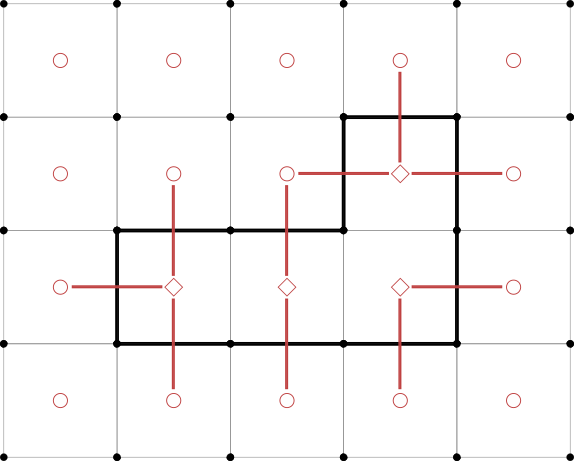
\includegraphics[width=0.5\textwidth]{./img/ising-graph.png}
		\end{center}
		\caption{An example of a closed graph $G$ in black and the corresponding graph $G'$ in red.}
		\label{fig:ising_graph}
	\end{figure}

	If we take the new graph $G'$ as a lattice with a set of spins $\{x_i\}$, strength of interaction $J$, and $\beta'$ representing the temperature, then the partition function of such a lattice defined by $G'$ is
	\begin{equation} \label{eq:PartitionFunction2DNewLattice}
		\begin{aligned}
			Z' &= \sum_{\{x_i\}} \prod_{\langle i,j \rangle} e^{\beta' J x_i x_j} \\
			&= \sum_{\{x_i\}} e^{-L\beta' J} \cdot e^{(2N-L)\beta' J} g(L) \\
			&= e^{2N\beta' J} \sum_{L} e^{-2L\beta' J} g(L)
		\end{aligned}
	\end{equation}
	where $g(L)$ is the number of ways to arrange $L$ edges in graph $G'$, which means the number of ways to arrange $L$ pairs of nearest neighbours $x_i=+1$ and $x_j=-1$.
	
	Considering the correspondence between $G$ and $G'$, we have $f(L) = g(L)$. Let $e^{-2\beta' J} = t$, remembering that $t = \tanh(\beta J)$. Join equations \eqref{eq:PartitionFunction2DTransformed} and \eqref{eq:PartitionFunction2DNewLattice}
	\begin{equation} \label{eq:PartitionFunction2DComparison}
		Z = 2^N \cosh^{2N}(\beta J) \tanh^{-N}(\beta J) Z'
	\end{equation}

	Now let's take $Z$ as a function of $\beta$, and $Z'$ as a function of $\beta'$. When $\beta$ is finite, $\beta' J = -\frac12 \ln{\tanh(\beta J)}$ is also finite. From equation \eqref{eq:PartitionFunction2DComparison}, we can see that if $Z(\beta)$ has a singularity at $\beta = \beta_c$, then $Z'(\beta')$ has a singularity at $\beta' = \beta'_c$.
	If we assume that there is only one critical temperature $T_c$, which means only one singularity, we will get
	\begin{equation} \label{eq:Singularity}
		\beta_c = \beta'_c
	\end{equation}

	Solution to equation \eqref{eq:CriticalTemperature} yields the critical temperature
	\begin{equation} \label{eq:CriticalTemperature}
		k_B T_c = \frac{2}{\ln(1+\sqrt{2})}J \approx 2.269J
	\end{equation}

	We have found $T_c$ of the 2D Ising model, but if we want to calculate the partition function, we still need to calculate out $f(L)$, which is a combinatorial problem. This is discussed in Feynman's book\cite{feynman1972statistical}.
	
	\subsection{Metropolis-Hastings Algorithm}
	\label{metropolis_algorithm}
	
	The Metropolis-Hastings algorithm is a Markov Chain Monte Carlo method used to sample from a probability distribution. In this case of the Ising model, the algorithm is as follows:
	\begin{enumerate}
		\item Choose a spin at random from the grid.
		\item Calculate the energy change $\Delta H$ if this spin were to flip.
		\item If $\Delta H \leq 0$ flip the spin, otherwise flip the spin with probability $e^{-\beta\Delta H}$.
		\item Repeat this process.
	\end{enumerate}

	To validate the algorithm, we shall prove that when the system reaches equilibrium, we will have a canonical ensemble, i.e. a probability distribution given by equation \eqref{eq:Probability}.\\
	
	Suppose we have an Ising model with $N$ spins. Let $A, B$ be two states of the system. The Markov Chain is described by a transition matrix $\pi$ with elements $\pi_{AB}$, which is the probability of transitioning from state $A$ to state $B$. Only when there is no more than one spin flipped between states $A$ and $B$ can $\pi_{AB}$ be non-zero. For such $A \neq B$, we have
	\begin{equation}
		\pi_{AB} = \begin{cases}
			\frac{1}{N} & H(A) \geq H(B) \\
			\frac{1}{N} e^{-\beta(H(B) - H(A))} & H(A) < H(B)
		\end{cases},
	\end{equation}
	and $\pi_{AA} = 1 - \sum_{B \neq A} \pi_{AB}$. When equilibrium is reached, for any two states $A, B$, we expect a balance of probability fluxes
	\begin{equation}
		P(A) \pi_{AB} = P(B) \pi_{BA}.
	\end{equation}
	By simplifying the above equation we get
	\begin{equation}
		\frac{P(A)}{P(B)} = \frac{\pi_{BA}}{\pi_{AB}} = \frac{e^{-\beta H(A)}}{e^{-\beta H(B)}}.
	\end{equation}
	Finally, introducing $\displaystyle Z = \sum_A e^{-\beta H(A)}$ for normalization
	\begin{equation}
		P(A) = \frac{e^{-\beta H(A)}}{Z},
	\end{equation}
	which is the canonical ensemble, therefore showing the algorithm is equivalent.

	\section{Implementation}
	
	The first step was to create a grid of spins. We chose to have the spins randomly distributed but with a bias towards the "up" direction. This ensured the magnetisation, which is sensitive to initial conditions, approached the same average each time.\\
	
	The next step is then to repeatedly apply the algorithm described in section \ref{metropolis_algorithm}. Starting in two dimensions, we ran some initial tests of the model to observe the behaviour of the spins as the algorithm iterates, as shown in figure \ref{fig:ising_grid}. This nicely demonstrates the tendency for groups of aligned spins to form.
	\begin{figure}[H]
		\begin{center}
			
\includegraphics[width=0.5\textwidth]{./img/ising-simulation.png}
		\end{center}
		\caption{A two-dimensional Ising Model simulation on a $500\times 500$ grid with parameters $\beta = 1.0$ and $h = 0$. The two colours correspond to the two different values of spin.}
		\label{fig:ising_grid}
	\end{figure}
	
	In order to find the temperature dependence of the energy, magnetisation and heat capacity, we needed to run the same simulation for a number of different values of $\beta$. Each simulation needs to be run for a sufficient number of iterations such that its mean values reach equilibrium. The energy and magnetisation will continue to change, but the average should approach a specific value. To test for this, we applied the following stopping condition:
	\begin{itemize}
		\item For each block of $n$ iterations:
		\begin{enumerate}
			\item Calculate the mean energy and magnetisation values for the current block.
			\item Compare the change of these mean values from the current block to those of the previous block.
			\item If both values have changed by less than three times the standard deviation of the mean $\displaystyle\left(\frac{\sigma}{\sqrt{n}}\right)$, it is considered to be at equilibrium and the simulation stops.
		\end{enumerate}
		\item There is also a set maximum iterations $N_\text{max}$ to ensure the algorithm doesn't continue ad infinitum.
	\end{itemize}
	It is important to ensure the block size $n$ is large enough that the probability of the stopping condition triggering erroneously is minimised. \\
	
	Once the simulation has finished for the range of temperature values, the calculated energy and magnetisation along with their respective temperatures are recorded in a CSV file. From the energy data, the heat capacity values can be calculated using $C_V = \frac{\partial E}{\partial T}$. To calculate this gradient, a least-square fit was used along small intervals of energy values, in order to estimate the gradient. This reduces errors from random variations in the calculated energy values.
	
	\section{Results}
	
	First, we ran a 2D simulation with grid size $1000 \times 1000$ and no external magnetic field, obtaining the results shown in figure \ref{fig:2d_1000_result}.
	\begin{figure}[H]
		\begin{subfigure}{\textwidth}
			\begin{center}
				\begin{tikzpicture}
					\begin{axis}[width=0.78\textwidth, height=0.47\textwidth, xlabel=$k_BT/J$, ylabel=$E/JN$]
						\addplot [mark size=0pt,blue] table[
						col sep=comma,
						x=temp,
						y=energy]
						{csv/onsager-energy.csv};
						
						\addplot [mark=*,mark size=0.5pt,black] table[
						col sep=comma,
						x=temp,
						y=energy,
						only marks]
						{csv/energy-1000.csv};
					\end{axis}
				\end{tikzpicture}
			\end{center}
			\caption{A plot showing average energy per particle against $k_BT$, both in units of the interaction strength $J$.}
		\end{subfigure}
	\end{figure}
	\begin{figure}[H]\ContinuedFloat
		\begin{subfigure}{0.45\textwidth}
			\begin{center}
				\begin{tikzpicture}
					\begin{axis}[width=\textwidth, height=0.7\textwidth, xlabel=$k_BT/J$, ylabel=$M/N$]
						\addplot [mark size=0pt,blue] table[
						col sep=comma,
						x=temp,
						y=magnetisation]
						{csv/onsager-magnetisation.csv};
						
						\addplot [mark=*,mark size=0.5pt,black] table[
						col sep=comma,
						x=temp,
						y=magnetisation,
						only marks]
						{csv/magnetisation-1000.csv};
					\end{axis}
				\end{tikzpicture}
			\end{center}
			\caption{A plot showing average magnetisation per particle against $k_BT$ in units of the interaction strength $J$.}
		\end{subfigure}
		\begin{subfigure}{0.45\textwidth}
			\begin{center}
				\begin{tikzpicture}
					\begin{axis}[width=\textwidth, height=0.7\textwidth, xlabel=$k_BT/J$, ylabel=$C_V/N$]
						\addplot [mark size=0pt,blue] table[
						col sep=comma,
						x=temp,
						y=heat-cap]
						{csv/onsager-heat-cap.csv};
						
						\addplot [mark=*,mark size=0.5pt,black] table[
						col sep=comma,
						x=temp,
						y=heat-cap,
						only marks]
						{csv/heat-cap-1000.csv};
					\end{axis}
				\end{tikzpicture}
			\end{center}
			\caption{A plot showing average heat capacity per particle against $k_BT$ in units of the interaction strength $J$.}
		\end{subfigure}
	
		\caption{Plots of data from a 2D Ising model simulation with grid size $1000 \times 1000$ and no external magnetic field. In each plot, the blue line is the expected result using Onsager's solution, and the black points are the data calculated by our simulation.}
		\label{fig:2d_1000_result}
	\end{figure}
	
	From these results we can see that they closely follow the exact solution, showing a phase change at $k_BT = k_BT_c \approx 2.269J$, indicating that using a Metropolis-Hastings algorithm is a successful method for predicting the behaviours of the model. The results for heat capacity don't have the same sharp peak as the exact solution. Since this peak tends to infinity in the exact solution, our value is limited by both the resolution of temperature values we were using in our simulation and the size of the grid. 
	
	\subsection{Two-dimensional Model with External Magnetic Field}
	
	Onsager's solution does not apply if there is an external magnetic field present. We tested a range of values for $h$ to compare the effect an external magnetic field has on the temperature dependence of magnetisation. These results are shown in figure \ref{fig:2d_mag_results}.
	\begin{figure}[H]
		\begin{center}
			\begin{tikzpicture}
				\begin{axis}[width=\textwidth, height=0.6\textwidth, xlabel=$k_BT/J$, ylabel=$M/N$]
					\addplot [mark=*,mark size=0.2pt,black] table[
					col sep=comma,
					x=temp,
					y=magnetisation,
					only marks]
					{csv/mag/magnetisation(-0.0).csv};
					\addlegendentry{$h = 0.0\;J$}
					
					\addplot [mark=*,mark size=0.2pt,orange] table[
					col sep=comma,
					x=temp,
					y=magnetisation,
					only marks]
					{csv/mag/magnetisation(-0.1).csv};
					\addlegendentry{$h = \pm0.1\;J$}
					
					\addplot [mark=*,mark size=0.2pt,blue] table[
					col sep=comma,
					x=temp,
					y=magnetisation,
					only marks]
					{csv/mag/magnetisation(-0.25).csv};
					\addlegendentry{$h = \pm0.25\;J$}
					
					\addplot [mark=*,mark size=0.2pt,green] table[
					col sep=comma,
					x=temp,
					y=magnetisation,
					only marks]
					{csv/mag/magnetisation(-0.5).csv};
					\addlegendentry{$h = \pm0.5\;J$}
					
					\addplot [mark=*,mark size=0.2pt,black] table[
					col sep=comma,
					x=temp,
					y=magnetisation,
					only marks]
					{csv/magnetisation-1000.csv};
					
					\addplot [mark=*,mark size=0.2pt,orange] table[
					col sep=comma,
					x=temp,
					y=magnetisation,
					only marks]
					{csv/mag/magnetisation(0.1).csv};
					
					\addplot [mark=*,mark size=0.2pt,blue] table[
					col sep=comma,
					x=temp,
					y=magnetisation,
					only marks]
					{csv/mag/magnetisation(0.25).csv};
					
					\addplot [mark=*,mark size=0.2pt,green] table[
					col sep=comma,
					x=temp,
					y=magnetisation,
					only marks]
					{csv/mag/magnetisation(0.5).csv};
				\end{axis}
			\end{tikzpicture}
		\end{center}
		\caption{Average magnetisation per particle against $k_BT$ for different values of external magnetic field $h$. For $h=0$ both positive and negative magnetisation are shown as they are both equally likely.}
		\label{fig:2d_mag_results}
	\end{figure}
	As an external magnetic field is applied, the model loses its phase change at $T_c$. Instead there is a more gradual decrease in average magnetisation as the temperature increases and the energy fluctuations also increase. As is to be expected, for higher values of $h$, this decrease becomes progressively slower. For $h=0$, the model is very sensitive to initial conditions and these are what will determine the final magnetisation state. 
	
	\section{Conclusion}
  
	In conclusion, while exact analytic solutions exist for some cases of the Ising model, using a Monte Carlo simulation to solve for its behaviours is both simpler and more easily extended. Our simulations correctly showed a phase change at $k_B T = k_BT_c \approx 2.269 J$ for $h=0$. We also went beyond the analytic solution, finding how the temperature dependence of magnetisation changes with different external magnetic fields. Our work could be extended by applying these same principles to a 3-dimensional model, which is more useful for most real-world systems.
	
	\bibliography{references} 

\end{document}